% !TEX root = ../master-thesis.tex



\begin{figure}
    \centering
    \addletter{140}{a}
    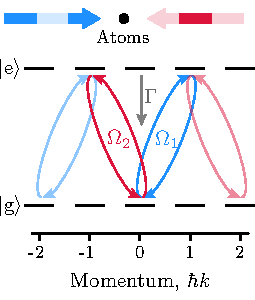
\includegraphics{fig-ai/ssh-scheme.pdf}
    \hfill
    \addletter{140}{b}
    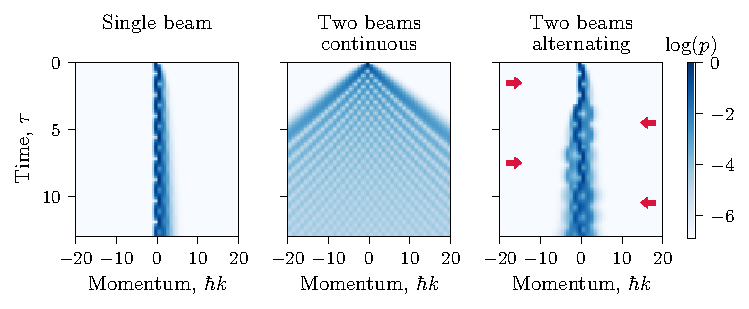
\includegraphics{fig-py/ssh-model.pdf}
    \caption{
        \textbf{Numerical simulation of momentum-space dynamics in the SSH model}. 
        a) Atoms undergo momentum-changing transitions via couplings $\Omega_1$ and $\Omega_2$, realizing a SSH-like quantum walk.
        b) Momentum distributions over time for different beam configurations: single beam (left) shows small shift; two continuous beams (middle) result in fast spreading; alternating beams (right) suppress spread.
    }
    \label{fig:sshmodel}
\end{figure}


Understanding the fundamental limitations and optimal strategies for free-space imaging requires a theoretical framework that captures the interplay between photon scattering, momentum transfer, and spatial resolution. This section develops a model based on the Su-Schrieffer-Heeger (SSH) Hamiltonian to explain the motivation for alternating beam sequences and to estimate the characteristic resolution limits of the imaging scheme.



\textbf{Recoil heating and momentum diffusion.} Although $^6$Li is a light atom and experiences relatively large momentum recoil during scattering, its broad D2 transition at $\lambda = 671$ nm allows for rapid photon emission. The typical recoil velocity is given by $v_\mathrm{rec} = h/(m\lambda)$, where $m$ is the atomic mass of $^6$Li and $\lambda$ is the wavelength of the imaging light. As the atom scatters photons at a rate $\Gamma$, each with random emission direction, it undergoes a random walk in momentum space, resulting in spatial diffusion during the imaging pulse.

The root-mean-square width of this random walk is approximately \cite{kruip_design_2024}
\begin{equation}
\sigma_\mathrm{rw} = \frac{1}{3} v_\mathrm{rec} \Gamma^{1/2} t^{3/2},
\label{eq:sigmarw}
\end{equation}
where $t$ is the total exposure time. For a fixed number of scattered photons $N_\mathrm{ph}$, we can express $t = N_\mathrm{ph}/\Gamma$, yielding
\begin{equation}
\sigma_\mathrm{rw} = \frac{1}{3} v_\mathrm{rec} \Gamma^{-1} N_\mathrm{ph}^{3/2}.
\end{equation}

This scaling highlights the trade-off between collecting more fluorescence photons and maintaining spatial resolution. In our system, with $N_\mathrm{ph} \approx 300$ scattered photons (of which approximately 10\% are detected by the camera), the resulting diffusion is on the scale of \red{10 $\mu$m}, which sets the practical limit for spatial resolution in free-space imaging of $^6$Li atoms.


\textbf{SSH model.} The scattering dynamics of a freely moving atom illuminated by resonant counter-propagating beams can be understood as a momentum-space quantum walk that maps onto the Su-Schrieffer-Heeger (SSH) model. In the standard SSH model, particles hop between two sublattices with alternating coupling strengths:
\begin{equation}
H = t_1 \sum_n |n,B\rangle \langle n,A| + t_2 \sum_n |n+1,A\rangle \langle n,B| + \text{h.c.}
\end{equation}

For the atomic case, this model takes the form:
\begin{equation}
H = \frac{\Omega_1}{2} \sum_p |p,g\rangle \langle p+1,e| + \frac{\Omega_2}{2} \sum_p |p-1,e\rangle \langle p,g| + \text{h.c.}
\end{equation}
where $\Omega_1$ and $\Omega_2$ correspond to the Rabi frequencies of the two counter-propagating beams, and $|p,g\rangle$ and $|p,e\rangle$ represent ground and excited states with momentum $p$.

A single beam produces systematic momentum transfer due to the finite linewidth $\Gamma$, leading to directed acceleration and displacement of the atomic cloud. When both beams are applied simultaneously, the atom undergoes coherent transitions between distant momentum states, resulting in rapid delocalization in space. This coherent coupling between momentum states separated by $2\hbar k$ leads to fast spreading of the momentum distribution.

The solution involves alternating the two beams rather than applying them simultaneously. This approach dramatically suppresses spatial diffusion by confining the coherent dynamics to simple oscillations between $\pm\hbar k$ states rather than allowing diffusion to higher momentum states. The evolution can be simulated by solving a Lindblad master equation:
\begin{equation}
i\hbar \partial_t \rho = [H(t), \rho] + \mathcal{L}[\rho],
\end{equation}
where $\mathcal{L}$ describes spontaneous emission. Numerical simulations demonstrate that alternating beam sequences significantly improve imaging fidelity compared to single-beam or simultaneous two-beam configurations (Fig.~\ref{fig:sshmodel}) as also was shown in \cite{su_fast_2025,bergschneider_spin-resolved_2018}.



The theoretical framework developed here provides the foundation for the experimental implementation described in the following sections, where the alternating beam protocol is realized using acousto-optic modulators.